\BourbakiUnnumberedChapter{Table}{Table}

Conventions (cf.~page IV, 66).

A symbol such as \(p^{\alpha} \cdot q^{\beta} \ldots\) , where \(p, q, \alpha, \beta, \ldots\) are integers \(\geqslant 1\) , denotes an element of \(D_{k}\) where \(k = p\alpha + q\beta + \cdots\) having \(\alpha\) components equal to \(p, \beta\) components equal to q, etc. Thus \(3 \cdot 1^{2}\) denotes the element of \(D_{5}\) equal to (3, 1, 1, 0, 0), while \(1^{4}\) denotes the element (1, 1, 1, 1) of \(D_{4}\) .

On the right of the row of index \(\alpha\) of the matrix \(C\) the expression of \(S(\alpha)\) as monomial in \(s_1, \ldots, s_k\) is given. For example, for \(k = 3\) and \(\alpha = 2.1\) we have

\[
\mathrm{S} (2. 1) = s _ {1} s _ {2} = \mathrm{M} (2. 1) + 3 \mathrm{M} \left(1 ^ {3}\right).
\]

We have used a corresponding convention for the columns of the matrix D. For example, for \(k = 4\) and \(\alpha = 2^2\) we have

\[
\mathbf {M} (2 ^ {2}) = 2 s _ {4} - 2 s _ {1} s _ {3} + s _ {2} ^ {2}.
\]

We recall that \(\mathbf{M}(2^2)\) is the sum of all monomials of the form \(\mathbf{X}_i^2\mathbf{X}_j^2\) for \(1 \leqslant i < j \leqslant n\) in the ring \(\mathbf{Z}[\mathbf{X}_1, \ldots, \mathbf{X}_n]\) .

An empty box indicates a zero element of the matrices C and D.

Matrix D\\
\(k = 2\)\\
\pandocbounded{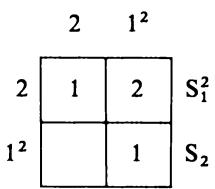
\includegraphics[keepaspectratio]{images/part001_666ab4c0.jpg}}

\pandocbounded{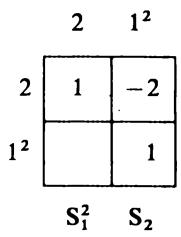
\includegraphics[keepaspectratio]{images/part001_442e375f.jpg}}

\(k = 3\)

3

2.1

\(1^{3}\)

3

1

3

6

\(S_{1}^{3}\)

2.1

1

3

\(S_{1}S_{2}\)

\(1^{3}\)

1

\(S_{3}\)

3 2.1 \(1^{3}\)\\
\pandocbounded{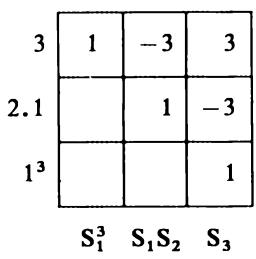
\includegraphics[keepaspectratio]{images/part001_fb1fe29f.jpg}}

\(k = 4\)

4

1

4

6

12

24

\(S_{1}^{4}\)

3.1

1

2

5

12

\(S_{1}^{2}S_{2}\)

\(2^{2}\)

1

2

6

\(S_{2}^{2}\)

\(2.1^{2}\)

1

4

\(S_{1}S_{3}\)

\(1^{4}\)

1

\(S_{4}\)

Matrix C

\pandocbounded{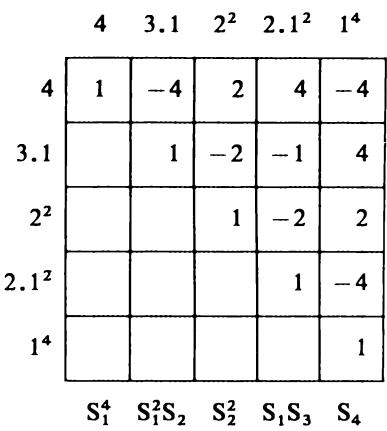
\includegraphics[keepaspectratio]{images/part001_bf35a948.jpg}}

\pandocbounded{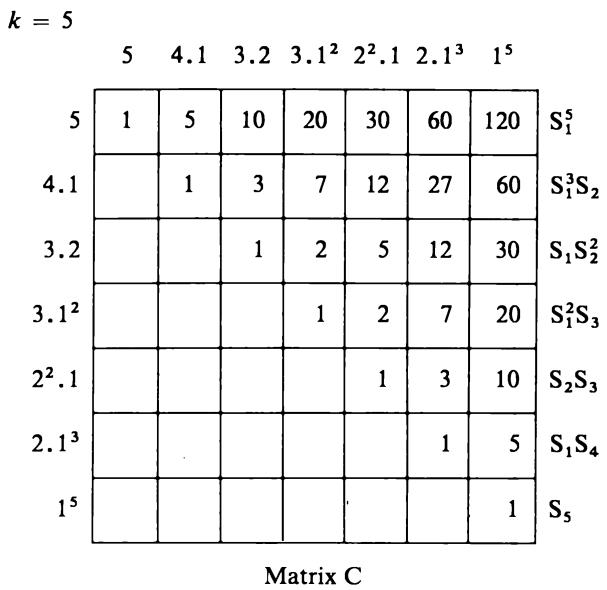
\includegraphics[keepaspectratio]{images/part001_7e862639.jpg}}

\pandocbounded{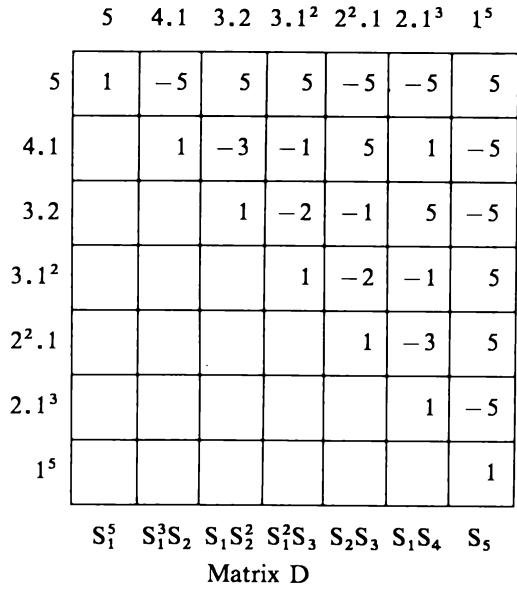
\includegraphics[keepaspectratio]{images/part001_eab66d56.jpg}}


